\documentclass[1p]{elsarticle_modified}
%\bibliographystyle{elsarticle-num}

%\usepackage[colorlinks]{hyperref}
%\usepackage{abbrmath_seonhwa} %\Abb, \Ascr, \Acal ,\Abf, \Afrak
\usepackage{amsfonts}
\usepackage{amssymb}
\usepackage{amsmath}
\usepackage{amsthm}
\usepackage{scalefnt}
\usepackage{amsbsy}
\usepackage{kotex}
\usepackage{caption}
\usepackage{subfig}
\usepackage{color}
\usepackage{graphicx}
\usepackage{xcolor} %% white, black, red, green, blue, cyan, magenta, yellow
\usepackage{float}
\usepackage{setspace}
\usepackage{hyperref}

\usepackage{tikz}
\usetikzlibrary{arrows}

\usepackage{multirow}
\usepackage{array} % fixed length table
\usepackage{hhline}

%%%%%%%%%%%%%%%%%%%%%
\makeatletter
\renewcommand*\env@matrix[1][\arraystretch]{%
	\edef\arraystretch{#1}%
	\hskip -\arraycolsep
	\let\@ifnextchar\new@ifnextchar
	\array{*\c@MaxMatrixCols c}}
\makeatother %https://tex.stackexchange.com/questions/14071/how-can-i-increase-the-line-spacing-in-a-matrix
%%%%%%%%%%%%%%%

\usepackage[normalem]{ulem}

\newcommand{\msout}[1]{\ifmmode\text{\sout{\ensuremath{#1}}}\else\sout{#1}\fi}
%SOURCE: \msout is \stkout macro in https://tex.stackexchange.com/questions/20609/strikeout-in-math-mode

\newcommand{\cancel}[1]{
	\ifmmode
	{\color{red}\msout{#1}}
	\else
	{\color{red}\sout{#1}}
	\fi
}

\newcommand{\add}[1]{
	{\color{blue}\uwave{#1}}
}

\newcommand{\replace}[2]{
	\ifmmode
	{\color{red}\msout{#1}}{\color{blue}\uwave{#2}}
	\else
	{\color{red}\sout{#1}}{\color{blue}\uwave{#2}}
	\fi
}

\newcommand{\Sol}{\mathcal{S}} %segment
\newcommand{\D}{D} %diagram
\newcommand{\A}{\mathcal{A}} %arc


%%%%%%%%%%%%%%%%%%%%%%%%%%%%%5 test

\def\sl{\operatorname{\textup{SL}}(2,\Cbb)}
\def\psl{\operatorname{\textup{PSL}}(2,\Cbb)}
\def\quan{\mkern 1mu \triangleright \mkern 1mu}

\theoremstyle{definition}
\newtheorem{thm}{Theorem}[section]
\newtheorem{prop}[thm]{Proposition}
\newtheorem{lem}[thm]{Lemma}
\newtheorem{ques}[thm]{Question}
\newtheorem{cor}[thm]{Corollary}
\newtheorem{defn}[thm]{Definition}
\newtheorem{exam}[thm]{Example}
\newtheorem{rmk}[thm]{Remark}
\newtheorem{alg}[thm]{Algorithm}

\newcommand{\I}{\sqrt{-1}}
\begin{document}

%\begin{frontmatter}
%
%\title{Boundary parabolic representations of knots up to 8 crossings}
%
%%% Group authors per affiliation:
%\author{Yunhi Cho} 
%\address{Department of Mathematics, University of Seoul, Seoul, Korea}
%\ead{yhcho@uos.ac.kr}
%
%
%\author{Seonhwa Kim} %\fnref{s_kim}}
%\address{Center for Geometry and Physics, Institute for Basic Science, Pohang, 37673, Korea}
%\ead{ryeona17@ibs.re.kr}
%
%\author{Hyuk Kim}
%\address{Department of Mathematical Sciences, Seoul National University, Seoul 08826, Korea}
%\ead{hyukkim@snu.ac.kr}
%
%\author{Seokbeom Yoon}
%\address{Department of Mathematical Sciences, Seoul National University, Seoul, 08826,  Korea}
%\ead{sbyoon15@snu.ac.kr}
%
%\begin{abstract}
%We find all boundary parabolic representation of knots up to 8 crossings.
%
%\end{abstract}
%\begin{keyword}
%    \MSC[2010] 57M25 
%\end{keyword}
%
%\end{frontmatter}

%\linenumbers
%\tableofcontents
%
\newcommand\colored[1]{\textcolor{white}{\rule[-0.35ex]{0.8em}{1.4ex}}\kern-0.8em\color{red} #1}%
%\newcommand\colored[1]{\textcolor{white}{ #1}\kern-2.17ex	\textcolor{white}{ #1}\kern-1.81ex	\textcolor{white}{ #1}\kern-2.15ex\color{red}#1	}

{\Large $\underline{12a_{0890}~(K12a_{0890})}$}

\setlength{\tabcolsep}{10pt}
\renewcommand{\arraystretch}{1.6}
\vspace{1cm}\begin{tabular}{m{100pt}>{\centering\arraybackslash}m{274pt}}
\multirow{5}{120pt}{
	\centering
	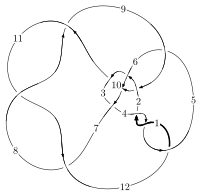
\includegraphics[width=112pt]{../../../GIT/diagram.site/Diagrams/png/1691_12a_0890.png}\\
\ \ \ A knot diagram\footnotemark}&
\allowdisplaybreaks
\textbf{Linearized knot diagam} \\
\cline{2-2}
 &
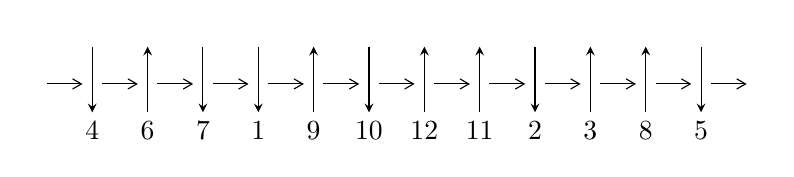
\begin{tikzpicture}[x=20pt, y=17pt]
	% nodes
	\node (C0) at (0, 0) {};
	\node (C1) at (1, 0) {};
	\node (C1U) at (1, +1) {};
	\node (C1D) at (1, -1) {4};

	\node (C2) at (2, 0) {};
	\node (C2U) at (2, +1) {};
	\node (C2D) at (2, -1) {6};

	\node (C3) at (3, 0) {};
	\node (C3U) at (3, +1) {};
	\node (C3D) at (3, -1) {7};

	\node (C4) at (4, 0) {};
	\node (C4U) at (4, +1) {};
	\node (C4D) at (4, -1) {1};

	\node (C5) at (5, 0) {};
	\node (C5U) at (5, +1) {};
	\node (C5D) at (5, -1) {9};

	\node (C6) at (6, 0) {};
	\node (C6U) at (6, +1) {};
	\node (C6D) at (6, -1) {10};

	\node (C7) at (7, 0) {};
	\node (C7U) at (7, +1) {};
	\node (C7D) at (7, -1) {12};

	\node (C8) at (8, 0) {};
	\node (C8U) at (8, +1) {};
	\node (C8D) at (8, -1) {11};

	\node (C9) at (9, 0) {};
	\node (C9U) at (9, +1) {};
	\node (C9D) at (9, -1) {2};

	\node (C10) at (10, 0) {};
	\node (C10U) at (10, +1) {};
	\node (C10D) at (10, -1) {3};

	\node (C11) at (11, 0) {};
	\node (C11U) at (11, +1) {};
	\node (C11D) at (11, -1) {8};

	\node (C12) at (12, 0) {};
	\node (C12U) at (12, +1) {};
	\node (C12D) at (12, -1) {5};
	\node (C13) at (13, 0) {};

	% arrows
	\draw[->,>={angle 60}]
	(C0) edge (C1) (C1) edge (C2) (C2) edge (C3) (C3) edge (C4) (C4) edge (C5) (C5) edge (C6) (C6) edge (C7) (C7) edge (C8) (C8) edge (C9) (C9) edge (C10) (C10) edge (C11) (C11) edge (C12) (C12) edge (C13) ;	\draw[->,>=stealth]
	(C1U) edge (C1D) (C2D) edge (C2U) (C3U) edge (C3D) (C4U) edge (C4D) (C5D) edge (C5U) (C6U) edge (C6D) (C7D) edge (C7U) (C8D) edge (C8U) (C9U) edge (C9D) (C10D) edge (C10U) (C11D) edge (C11U) (C12U) edge (C12D) ;
	\end{tikzpicture} \\
\hhline{~~} \\& 
\textbf{Solving Sequence} \\ \cline{2-2} 
 &
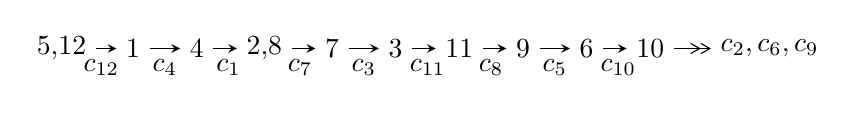
\begin{tikzpicture}[x=23pt, y=7pt]
	% node
	\node (A0) at (-1/8, 0) {5,12};
	\node (A1) at (1, 0) {1};
	\node (A2) at (2, 0) {4};
	\node (A3) at (49/16, 0) {2,8};
	\node (A4) at (33/8, 0) {7};
	\node (A5) at (41/8, 0) {3};
	\node (A6) at (49/8, 0) {11};
	\node (A7) at (57/8, 0) {9};
	\node (A8) at (65/8, 0) {6};
	\node (A9) at (73/8, 0) {10};
	\node (C1) at (1/2, -1) {$c_{12}$};
	\node (C2) at (3/2, -1) {$c_{4}$};
	\node (C3) at (5/2, -1) {$c_{1}$};
	\node (C4) at (29/8, -1) {$c_{7}$};
	\node (C5) at (37/8, -1) {$c_{3}$};
	\node (C6) at (45/8, -1) {$c_{11}$};
	\node (C7) at (53/8, -1) {$c_{8}$};
	\node (C8) at (61/8, -1) {$c_{5}$};
	\node (C9) at (69/8, -1) {$c_{10}$};
	\node (A10) at (11, 0) {$c_{2},c_{6},c_{9}$};

	% edge
	\draw[->,>=stealth]	
	(A0) edge (A1) (A1) edge (A2) (A2) edge (A3) (A3) edge (A4) (A4) edge (A5) (A5) edge (A6) (A6) edge (A7) (A7) edge (A8) (A8) edge (A9) ;
	\draw[->>,>={angle 60}]	
	(A9) edge (A10);
\end{tikzpicture} \\ 

\end{tabular} \\

\footnotetext{
The image of knot diagram is generated by the software ``\textbf{Draw programme}" developed by Andrew Bartholomew(\url{http://www.layer8.co.uk/maths/draw/index.htm\#Running-draw}), where we modified some parts for our purpose(\url{https://github.com/CATsTAILs/LinksPainter}).
}\phantom \\ \newline 
\centering \textbf{Ideals for irreducible components\footnotemark of $X_{\text{par}}$} 
 
\begin{align*}
I^u_{1}&=\langle 
-1.41774\times10^{373} u^{131}-8.81640\times10^{374} u^{130}+\cdots+2.89015\times10^{375} b-3.34965\times10^{375},\\
\phantom{I^u_{1}}&\phantom{= \langle  }-2.99895\times10^{379} u^{131}+1.52950\times10^{380} u^{130}+\cdots+9.38806\times10^{379} a-2.25117\times10^{380},\\
\phantom{I^u_{1}}&\phantom{= \langle  }u^{132}-5 u^{131}+\cdots+157 u+11\rangle \\
I^u_{2}&=\langle 
- u^{28}+7 u^{27}+\cdots+b-4,\;u^{29}-7 u^{28}+\cdots+a-5,\;u^{30}-6 u^{29}+\cdots-8 u+1\rangle \\
\\
\end{align*}
\raggedright * 2 irreducible components of $\dim_{\mathbb{C}}=0$, with total 162 representations.\\
\footnotetext{All coefficients of polynomials are rational numbers. But the coefficients are sometimes approximated in decimal forms when there is not enough margin.}
\newpage
\renewcommand{\arraystretch}{1}
\centering \section*{I. $I^u_{1}= \langle -1.42\times10^{373} u^{131}-8.82\times10^{374} u^{130}+\cdots+2.89\times10^{375} b-3.35\times10^{375},\;-3.00\times10^{379} u^{131}+1.53\times10^{380} u^{130}+\cdots+9.39\times10^{379} a-2.25\times10^{380},\;u^{132}-5 u^{131}+\cdots+157 u+11 \rangle$}
\flushleft \textbf{(i) Arc colorings}\\
\begin{tabular}{m{7pt} m{180pt} m{7pt} m{180pt} }
\flushright $a_{5}=$&$\begin{pmatrix}0\\u\end{pmatrix}$ \\
\flushright $a_{12}=$&$\begin{pmatrix}1\\0\end{pmatrix}$ \\
\flushright $a_{1}=$&$\begin{pmatrix}1\\u^2\end{pmatrix}$ \\
\flushright $a_{4}=$&$\begin{pmatrix}u\\u^3+u\end{pmatrix}$ \\
\flushright $a_{2}=$&$\begin{pmatrix}u^2+1\\u^4+2 u^2\end{pmatrix}$ \\
\flushright $a_{8}=$&$\begin{pmatrix}0.319443 u^{131}-1.62920 u^{130}+\cdots+0.0910581 u+2.39791\\0.00490543 u^{131}+0.305050 u^{130}+\cdots+19.2159 u+1.15899\end{pmatrix}$ \\
\flushright $a_{7}=$&$\begin{pmatrix}0.314537 u^{131}-1.93425 u^{130}+\cdots-19.1248 u+1.23892\\0.00490543 u^{131}+0.305050 u^{130}+\cdots+19.2159 u+1.15899\end{pmatrix}$ \\
\flushright $a_{3}=$&$\begin{pmatrix}-0.223257 u^{131}+0.637786 u^{130}+\cdots-10.4923 u-1.09005\\0.177227 u^{131}-0.982312 u^{130}+\cdots+5.69063 u+0.367339\end{pmatrix}$ \\
\flushright $a_{11}=$&$\begin{pmatrix}0.0674859 u^{131}-0.538029 u^{130}+\cdots-86.2553 u-6.81104\\-0.156492 u^{131}+1.20733 u^{130}+\cdots+16.5322 u-0.189296\end{pmatrix}$ \\
\flushright $a_{9}=$&$\begin{pmatrix}0.314728 u^{131}-1.46910 u^{130}+\cdots-68.2386 u-7.22115\\-0.293356 u^{131}+1.92375 u^{130}+\cdots+13.9230 u-0.672299\end{pmatrix}$ \\
\flushright $a_{6}=$&$\begin{pmatrix}0.367934 u^{131}-1.46158 u^{130}+\cdots+90.0780 u+9.93414\\0.187553 u^{131}-0.598991 u^{130}+\cdots+32.7497 u+2.66066\end{pmatrix}$ \\
\flushright $a_{10}=$&$\begin{pmatrix}0.518800 u^{131}-2.71076 u^{130}+\cdots-60.9506 u-5.07052\\-0.121163 u^{131}+1.13129 u^{130}+\cdots+25.4701 u+0.131622\end{pmatrix}$\\&\end{tabular}
\flushleft \textbf{(ii) Obstruction class $= -1$}\\~\\
\flushleft \textbf{(iii) Cusp Shapes $= 1.44696 u^{131}-9.05081 u^{130}+\cdots-486.405 u-47.5445$}\\~\\
\newpage\renewcommand{\arraystretch}{1}
\flushleft \textbf{(iv) u-Polynomials at the component}\newline \\
\begin{tabular}{m{50pt}|m{274pt}}
Crossings & \hspace{64pt}u-Polynomials at each crossing \\
\hline $$\begin{aligned}c_{1},c_{4},c_{12}\end{aligned}$$&$\begin{aligned}
&u^{132}+5 u^{131}+\cdots-157 u+11
\end{aligned}$\\
\hline $$\begin{aligned}c_{2}\end{aligned}$$&$\begin{aligned}
&u^{132}-3 u^{131}+\cdots-20 u+1
\end{aligned}$\\
\hline $$\begin{aligned}c_{3}\end{aligned}$$&$\begin{aligned}
&u^{132}-2 u^{131}+\cdots+768008 u-38548
\end{aligned}$\\
\hline $$\begin{aligned}c_{5}\end{aligned}$$&$\begin{aligned}
&u^{132}+2 u^{131}+\cdots-768008 u-38548
\end{aligned}$\\
\hline $$\begin{aligned}c_{6}\end{aligned}$$&$\begin{aligned}
&u^{132}+3 u^{131}+\cdots+20 u+1
\end{aligned}$\\
\hline $$\begin{aligned}c_{7},c_{8},c_{11}\end{aligned}$$&$\begin{aligned}
&u^{132}-5 u^{131}+\cdots+157 u+11
\end{aligned}$\\
\hline $$\begin{aligned}c_{9}\end{aligned}$$&$\begin{aligned}
&u^{132}- u^{131}+\cdots+123 u-5
\end{aligned}$\\
\hline $$\begin{aligned}c_{10}\end{aligned}$$&$\begin{aligned}
&u^{132}+u^{131}+\cdots-123 u-5
\end{aligned}$\\
\hline
\end{tabular}\\~\\
\newpage\renewcommand{\arraystretch}{1}
\flushleft \textbf{(v) Riley Polynomials at the component}\newline \\
\begin{tabular}{m{50pt}|m{274pt}}
Crossings & \hspace{64pt}Riley Polynomials at each crossing \\
\hline $$\begin{aligned}c_{1},c_{4},c_{7}\\c_{8},c_{11},c_{12}\end{aligned}$$&$\begin{aligned}
&y^{132}+125 y^{131}+\cdots-14859 y+121
\end{aligned}$\\
\hline $$\begin{aligned}c_{2},c_{6}\end{aligned}$$&$\begin{aligned}
&y^{132}- y^{131}+\cdots-208 y+1
\end{aligned}$\\
\hline $$\begin{aligned}c_{3},c_{5}\end{aligned}$$&$\begin{aligned}
&y^{132}-6 y^{131}+\cdots-24158727920 y+1485948304
\end{aligned}$\\
\hline $$\begin{aligned}c_{9},c_{10}\end{aligned}$$&$\begin{aligned}
&y^{132}+9 y^{131}+\cdots+571 y+25
\end{aligned}$\\
\hline
\end{tabular}\\~\\
\newpage\flushleft \textbf{(vi) Complex Volumes and Cusp Shapes}
$$\begin{array}{c|c|c}  
\text{Solutions to }I^u_{1}& \I (\text{vol} + \sqrt{-1}CS) & \text{Cusp shape}\\
 \hline 
\begin{aligned}
u &= -0.950162 + 0.371930 I \\
a &= \phantom{-}0.67877 - 2.14159 I \\
b &= -0.29964 - 1.46694 I\end{aligned}
 & -5.9520 + 14.1469 I & \phantom{-0.000000 } 0 \\ \hline\begin{aligned}
u &= -0.950162 - 0.371930 I \\
a &= \phantom{-}0.67877 + 2.14159 I \\
b &= -0.29964 + 1.46694 I\end{aligned}
 & -5.9520 - 14.1469 I & \phantom{-0.000000 } 0 \\ \hline\begin{aligned}
u &= -0.644129 + 0.714770 I \\
a &= -0.257686 - 0.441199 I \\
b &= -0.572702 + 0.256387 I\end{aligned}
 & \phantom{-}0.99836 - 5.34745 I & \phantom{-0.000000 } 0 \\ \hline\begin{aligned}
u &= -0.644129 - 0.714770 I \\
a &= -0.257686 + 0.441199 I \\
b &= -0.572702 - 0.256387 I\end{aligned}
 & \phantom{-}0.99836 + 5.34745 I & \phantom{-0.000000 } 0 \\ \hline\begin{aligned}
u &= \phantom{-}0.641102 + 0.836655 I \\
a &= \phantom{-}0.217211 - 0.127517 I \\
b &= -0.1095870 - 0.0579846 I\end{aligned}
 & -0.68851 - 2.45836 I & \phantom{-0.000000 } 0 \\ \hline\begin{aligned}
u &= \phantom{-}0.641102 - 0.836655 I \\
a &= \phantom{-}0.217211 + 0.127517 I \\
b &= -0.1095870 + 0.0579846 I\end{aligned}
 & -0.68851 + 2.45836 I & \phantom{-0.000000 } 0 \\ \hline\begin{aligned}
u &= \phantom{-}1.009860 + 0.421402 I \\
a &= \phantom{-}0.86690 + 2.04670 I \\
b &= -0.196199 + 1.388130 I\end{aligned}
 & -6.61469 - 4.90913 I & \phantom{-0.000000 } 0 \\ \hline\begin{aligned}
u &= \phantom{-}1.009860 - 0.421402 I \\
a &= \phantom{-}0.86690 - 2.04670 I \\
b &= -0.196199 - 1.388130 I\end{aligned}
 & -6.61469 + 4.90913 I & \phantom{-0.000000 } 0 \\ \hline\begin{aligned}
u &= \phantom{-}1.041540 + 0.340102 I \\
a &= -0.28770 - 2.08179 I \\
b &= \phantom{-}0.15746 - 1.43693 I\end{aligned}
 & -6.95360 - 4.28613 I & \phantom{-0.000000 } 0 \\ \hline\begin{aligned}
u &= \phantom{-}1.041540 - 0.340102 I \\
a &= -0.28770 + 2.08179 I \\
b &= \phantom{-}0.15746 + 1.43693 I\end{aligned}
 & -6.95360 + 4.28613 I & \phantom{-0.000000 } 0\\
 \hline 
 \end{array}$$\newpage$$\begin{array}{c|c|c}  
\text{Solutions to }I^u_{1}& \I (\text{vol} + \sqrt{-1}CS) & \text{Cusp shape}\\
 \hline 
\begin{aligned}
u &= \phantom{-}0.440285 + 1.014920 I \\
a &= -0.099470 - 0.884634 I \\
b &= -0.101752 - 1.377020 I\end{aligned}
 & -3.06770 - 1.78673 I & \phantom{-0.000000 } 0 \\ \hline\begin{aligned}
u &= \phantom{-}0.440285 - 1.014920 I \\
a &= -0.099470 + 0.884634 I \\
b &= -0.101752 + 1.377020 I\end{aligned}
 & -3.06770 + 1.78673 I & \phantom{-0.000000 } 0 \\ \hline\begin{aligned}
u &= \phantom{-}0.766251 + 0.455073 I \\
a &= \phantom{-}0.265973 + 0.448281 I \\
b &= -0.470216 + 0.263747 I\end{aligned}
 & -1.37915 - 2.38176 I & \phantom{-0.000000 } 0 \\ \hline\begin{aligned}
u &= \phantom{-}0.766251 - 0.455073 I \\
a &= \phantom{-}0.265973 - 0.448281 I \\
b &= -0.470216 - 0.263747 I\end{aligned}
 & -1.37915 + 2.38176 I & \phantom{-0.000000 } 0 \\ \hline\begin{aligned}
u &= -0.272305 + 0.846012 I \\
a &= \phantom{-}0.99449 - 1.05089 I \\
b &= \phantom{-}0.142486 - 1.394290 I\end{aligned}
 & -2.97007 - 2.46429 I & \phantom{-0.000000 } 0 \\ \hline\begin{aligned}
u &= -0.272305 - 0.846012 I \\
a &= \phantom{-}0.99449 + 1.05089 I \\
b &= \phantom{-}0.142486 + 1.394290 I\end{aligned}
 & -2.97007 + 2.46429 I & \phantom{-0.000000 } 0 \\ \hline\begin{aligned}
u &= -0.002790 + 1.111980 I \\
a &= \phantom{-}1.200990 + 0.179105 I \\
b &= -0.679439 - 0.185346 I\end{aligned}
 & \phantom{-}1.10025 - 3.05463 I & \phantom{-0.000000 } 0 \\ \hline\begin{aligned}
u &= -0.002790 - 1.111980 I \\
a &= \phantom{-}1.200990 - 0.179105 I \\
b &= -0.679439 + 0.185346 I\end{aligned}
 & \phantom{-}1.10025 + 3.05463 I & \phantom{-0.000000 } 0 \\ \hline\begin{aligned}
u &= \phantom{-}0.701907 + 0.537816 I \\
a &= -0.65478 - 1.73712 I \\
b &= \phantom{-}0.24496 - 1.47272 I\end{aligned}
 & -5.26519 - 5.78083 I & \phantom{-0.000000 } 0 \\ \hline\begin{aligned}
u &= \phantom{-}0.701907 - 0.537816 I \\
a &= -0.65478 + 1.73712 I \\
b &= \phantom{-}0.24496 + 1.47272 I\end{aligned}
 & -5.26519 + 5.78083 I & \phantom{-0.000000 } 0\\
 \hline 
 \end{array}$$\newpage$$\begin{array}{c|c|c}  
\text{Solutions to }I^u_{1}& \I (\text{vol} + \sqrt{-1}CS) & \text{Cusp shape}\\
 \hline 
\begin{aligned}
u &= -0.787382 + 0.386839 I \\
a &= -0.171210 - 0.646264 I \\
b &= -0.787382 - 0.386839 I\end{aligned}
 & \phantom{-0.000000 -}10.2016 I & \phantom{-0.000000 } 0 \\ \hline\begin{aligned}
u &= -0.787382 - 0.386839 I \\
a &= -0.171210 + 0.646264 I \\
b &= -0.787382 + 0.386839 I\end{aligned}
 & \phantom{-0.000000 } -10.2016 I & \phantom{-0.000000 } 0 \\ \hline\begin{aligned}
u &= \phantom{-}0.790592 + 0.347184 I \\
a &= \phantom{-}1.18615 + 1.90823 I \\
b &= \phantom{-}0.088744 + 1.394760 I\end{aligned}
 & -5.92340 + 0.99720 I & \phantom{-0.000000 } 0 \\ \hline\begin{aligned}
u &= \phantom{-}0.790592 - 0.347184 I \\
a &= \phantom{-}1.18615 - 1.90823 I \\
b &= \phantom{-}0.088744 - 1.394760 I\end{aligned}
 & -5.92340 - 0.99720 I & \phantom{-0.000000 } 0 \\ \hline\begin{aligned}
u &= \phantom{-}0.687351 + 0.513075 I \\
a &= \phantom{-}0.176990 - 0.369508 I \\
b &= \phantom{-}0.262179 - 0.400166 I\end{aligned}
 & -1.07235 - 2.41410 I & \phantom{-0.000000 } 0 \\ \hline\begin{aligned}
u &= \phantom{-}0.687351 - 0.513075 I \\
a &= \phantom{-}0.176990 + 0.369508 I \\
b &= \phantom{-}0.262179 + 0.400166 I\end{aligned}
 & -1.07235 + 2.41410 I & \phantom{-0.000000 } 0 \\ \hline\begin{aligned}
u &= \phantom{-}0.834729 + 0.037542 I \\
a &= \phantom{-}0.71946 + 2.02214 I \\
b &= -0.237782 + 1.365960 I\end{aligned}
 & -6.14153 - 2.77490 I & \phantom{-0.000000 } 0 \\ \hline\begin{aligned}
u &= \phantom{-}0.834729 - 0.037542 I \\
a &= \phantom{-}0.71946 - 2.02214 I \\
b &= -0.237782 - 1.365960 I\end{aligned}
 & -6.14153 + 2.77490 I & \phantom{-0.000000 } 0 \\ \hline\begin{aligned}
u &= -0.052414 + 1.189960 I \\
a &= \phantom{-}0.19582 - 1.80357 I \\
b &= \phantom{-}0.09579 - 1.60665 I\end{aligned}
 & -5.54517 - 3.33256 I & \phantom{-0.000000 } 0 \\ \hline\begin{aligned}
u &= -0.052414 - 1.189960 I \\
a &= \phantom{-}0.19582 + 1.80357 I \\
b &= \phantom{-}0.09579 + 1.60665 I\end{aligned}
 & -5.54517 + 3.33256 I & \phantom{-0.000000 } 0\\
 \hline 
 \end{array}$$\newpage$$\begin{array}{c|c|c}  
\text{Solutions to }I^u_{1}& \I (\text{vol} + \sqrt{-1}CS) & \text{Cusp shape}\\
 \hline 
\begin{aligned}
u &= -0.779630 + 0.926682 I \\
a &= -0.49471 + 1.36858 I \\
b &= -0.22434 + 1.40772 I\end{aligned}
 & -4.35497 - 8.28767 I & \phantom{-0.000000 } 0 \\ \hline\begin{aligned}
u &= -0.779630 - 0.926682 I \\
a &= -0.49471 - 1.36858 I \\
b &= -0.22434 - 1.40772 I\end{aligned}
 & -4.35497 + 8.28767 I & \phantom{-0.000000 } 0 \\ \hline\begin{aligned}
u &= -0.725162 + 0.248821 I \\
a &= -0.70693 + 2.63897 I \\
b &= \phantom{-}0.29518 + 1.48566 I\end{aligned}
 & -4.85475 + 6.28492 I & \phantom{-0.000000 } 0 \\ \hline\begin{aligned}
u &= -0.725162 - 0.248821 I \\
a &= -0.70693 - 2.63897 I \\
b &= \phantom{-}0.29518 - 1.48566 I\end{aligned}
 & -4.85475 - 6.28492 I & \phantom{-0.000000 } 0 \\ \hline\begin{aligned}
u &= \phantom{-}0.773343 + 0.965987 I \\
a &= -0.20955 - 1.69076 I \\
b &= -0.111989 - 1.330050 I\end{aligned}
 & -5.07572 - 1.26184 I & \phantom{-0.000000 } 0 \\ \hline\begin{aligned}
u &= \phantom{-}0.773343 - 0.965987 I \\
a &= -0.20955 + 1.69076 I \\
b &= -0.111989 + 1.330050 I\end{aligned}
 & -5.07572 + 1.26184 I & \phantom{-0.000000 } 0 \\ \hline\begin{aligned}
u &= -0.127151 + 1.235070 I \\
a &= -0.274968 + 1.030680 I \\
b &= -0.00337 + 1.71364 I\end{aligned}
 & -5.60110 + 5.35321 I & \phantom{-0.000000 } 0 \\ \hline\begin{aligned}
u &= -0.127151 - 1.235070 I \\
a &= -0.274968 - 1.030680 I \\
b &= -0.00337 - 1.71364 I\end{aligned}
 & -5.60110 - 5.35321 I & \phantom{-0.000000 } 0 \\ \hline\begin{aligned}
u &= \phantom{-}0.302620 + 0.682286 I \\
a &= \phantom{-}0.90325 + 1.10435 I \\
b &= -0.469146 + 0.011108 I\end{aligned}
 & \phantom{-}0.98745 - 3.37772 I & \phantom{-0.000000 } 0 \\ \hline\begin{aligned}
u &= \phantom{-}0.302620 - 0.682286 I \\
a &= \phantom{-}0.90325 - 1.10435 I \\
b &= -0.469146 - 0.011108 I\end{aligned}
 & \phantom{-}0.98745 + 3.37772 I & \phantom{-0.000000 } 0\\
 \hline 
 \end{array}$$\newpage$$\begin{array}{c|c|c}  
\text{Solutions to }I^u_{1}& \I (\text{vol} + \sqrt{-1}CS) & \text{Cusp shape}\\
 \hline 
\begin{aligned}
u &= \phantom{-}0.294316 + 1.220750 I \\
a &= \phantom{-}1.71095 + 0.48410 I \\
b &= -0.338573 + 1.267650 I\end{aligned}
 & -2.36146 - 6.82792 I & \phantom{-0.000000 } 0 \\ \hline\begin{aligned}
u &= \phantom{-}0.294316 - 1.220750 I \\
a &= \phantom{-}1.71095 - 0.48410 I \\
b &= -0.338573 - 1.267650 I\end{aligned}
 & -2.36146 + 6.82792 I & \phantom{-0.000000 } 0 \\ \hline\begin{aligned}
u &= \phantom{-}0.071265 + 1.261830 I \\
a &= -2.60204 - 0.77989 I \\
b &= \phantom{-}0.071265 - 1.261830 I\end{aligned}
 & \phantom{-0.000000 -}3.91086 I & \phantom{-0.000000 } 0 \\ \hline\begin{aligned}
u &= \phantom{-}0.071265 - 1.261830 I \\
a &= -2.60204 + 0.77989 I \\
b &= \phantom{-}0.071265 + 1.261830 I\end{aligned}
 & \phantom{-0.000000 } -3.91086 I & \phantom{-0.000000 } 0 \\ \hline\begin{aligned}
u &= -0.019111 + 1.286080 I \\
a &= -1.40117 + 0.89564 I \\
b &= \phantom{-}0.32094 + 1.40919 I\end{aligned}
 & \phantom{-}0.40947 + 3.05315 I & \phantom{-0.000000 } 0 \\ \hline\begin{aligned}
u &= -0.019111 - 1.286080 I \\
a &= -1.40117 - 0.89564 I \\
b &= \phantom{-}0.32094 - 1.40919 I\end{aligned}
 & \phantom{-}0.40947 - 3.05315 I & \phantom{-0.000000 } 0 \\ \hline\begin{aligned}
u &= -0.679439 + 0.185346 I \\
a &= \phantom{-}0.21866 - 3.01638 I \\
b &= -0.002790 - 1.111980 I\end{aligned}
 & -1.10025 - 3.05463 I & -1.25318 + 2.55597 I \\ \hline\begin{aligned}
u &= -0.679439 - 0.185346 I \\
a &= \phantom{-}0.21866 + 3.01638 I \\
b &= -0.002790 + 1.111980 I\end{aligned}
 & -1.10025 + 3.05463 I & -1.25318 - 2.55597 I \\ \hline\begin{aligned}
u &= \phantom{-}0.172704 + 1.295630 I \\
a &= \phantom{-}0.766858 - 0.146636 I \\
b &= -0.139306 - 0.387149 I\end{aligned}
 & \phantom{-}2.76297 - 2.67751 I & \phantom{-0.000000 } 0 \\ \hline\begin{aligned}
u &= \phantom{-}0.172704 - 1.295630 I \\
a &= \phantom{-}0.766858 + 0.146636 I \\
b &= -0.139306 + 0.387149 I\end{aligned}
 & \phantom{-}2.76297 + 2.67751 I & \phantom{-0.000000 } 0\\
 \hline 
 \end{array}$$\newpage$$\begin{array}{c|c|c}  
\text{Solutions to }I^u_{1}& \I (\text{vol} + \sqrt{-1}CS) & \text{Cusp shape}\\
 \hline 
\begin{aligned}
u &= -0.338573 + 1.267650 I \\
a &= -1.36573 + 1.59518 I \\
b &= \phantom{-}0.294316 + 1.220750 I\end{aligned}
 & \phantom{-}2.36146 + 6.82792 I & \phantom{-0.000000 } 0 \\ \hline\begin{aligned}
u &= -0.338573 - 1.267650 I \\
a &= -1.36573 - 1.59518 I \\
b &= \phantom{-}0.294316 - 1.220750 I\end{aligned}
 & \phantom{-}2.36146 - 6.82792 I & \phantom{-0.000000 } 0 \\ \hline\begin{aligned}
u &= -0.111989 + 1.330050 I \\
a &= -0.261450 + 0.227264 I \\
b &= \phantom{-}0.773343 - 0.965987 I\end{aligned}
 & \phantom{-}5.07572 - 1.26184 I & \phantom{-0.000000 } 0 \\ \hline\begin{aligned}
u &= -0.111989 - 1.330050 I \\
a &= -0.261450 - 0.227264 I \\
b &= \phantom{-}0.773343 + 0.965987 I\end{aligned}
 & \phantom{-}5.07572 + 1.26184 I & \phantom{-0.000000 } 0 \\ \hline\begin{aligned}
u &= -0.111538 + 1.333150 I \\
a &= -1.72458 - 0.02068 I \\
b &= \phantom{-}0.379857 + 0.270762 I\end{aligned}
 & \phantom{-}3.16255 + 5.26546 I & \phantom{-0.000000 } 0 \\ \hline\begin{aligned}
u &= -0.111538 - 1.333150 I \\
a &= -1.72458 + 0.02068 I \\
b &= \phantom{-}0.379857 - 0.270762 I\end{aligned}
 & \phantom{-}3.16255 - 5.26546 I & \phantom{-0.000000 } 0 \\ \hline\begin{aligned}
u &= -0.243111 + 1.317630 I \\
a &= \phantom{-}1.299540 - 0.408836 I \\
b &= -0.23465 - 1.42006 I\end{aligned}
 & -4.23968 + 0.21376 I & \phantom{-0.000000 } 0 \\ \hline\begin{aligned}
u &= -0.243111 - 1.317630 I \\
a &= \phantom{-}1.299540 + 0.408836 I \\
b &= -0.23465 + 1.42006 I\end{aligned}
 & -4.23968 - 0.21376 I & \phantom{-0.000000 } 0 \\ \hline\begin{aligned}
u &= \phantom{-}0.863385 + 1.032350 I \\
a &= \phantom{-}0.65186 + 1.42280 I \\
b &= \phantom{-}0.051249 + 1.356350 I\end{aligned}
 & -5.02593 - 2.17382 I & \phantom{-0.000000 } 0 \\ \hline\begin{aligned}
u &= \phantom{-}0.863385 - 1.032350 I \\
a &= \phantom{-}0.65186 - 1.42280 I \\
b &= \phantom{-}0.051249 - 1.356350 I\end{aligned}
 & -5.02593 + 2.17382 I & \phantom{-0.000000 } 0\\
 \hline 
 \end{array}$$\newpage$$\begin{array}{c|c|c}  
\text{Solutions to }I^u_{1}& \I (\text{vol} + \sqrt{-1}CS) & \text{Cusp shape}\\
 \hline 
\begin{aligned}
u &= \phantom{-}0.051249 + 1.356350 I \\
a &= -0.511244 + 0.312428 I \\
b &= \phantom{-}0.863385 + 1.032350 I\end{aligned}
 & \phantom{-}5.02593 + 2.17382 I & \phantom{-0.000000 } 0 \\ \hline\begin{aligned}
u &= \phantom{-}0.051249 - 1.356350 I \\
a &= -0.511244 - 0.312428 I \\
b &= \phantom{-}0.863385 - 1.032350 I\end{aligned}
 & \phantom{-}5.02593 - 2.17382 I & \phantom{-0.000000 } 0 \\ \hline\begin{aligned}
u &= \phantom{-}0.628407 + 0.055866 I \\
a &= \phantom{-}0.410455 - 0.178720 I \\
b &= -0.402004 - 0.116007 I\end{aligned}
 & -1.404620 - 0.021852 I & -7.39206 - 0.48985 I \\ \hline\begin{aligned}
u &= \phantom{-}0.628407 - 0.055866 I \\
a &= \phantom{-}0.410455 + 0.178720 I \\
b &= -0.402004 + 0.116007 I\end{aligned}
 & -1.404620 + 0.021852 I & -7.39206 + 0.48985 I \\ \hline\begin{aligned}
u &= -0.572702 + 0.256387 I \\
a &= -0.009101 + 1.173680 I \\
b &= -0.644129 + 0.714770 I\end{aligned}
 & -0.99836 + 5.34745 I & -2.97606 - 6.12125 I \\ \hline\begin{aligned}
u &= -0.572702 - 0.256387 I \\
a &= -0.009101 - 1.173680 I \\
b &= -0.644129 - 0.714770 I\end{aligned}
 & -0.99836 - 5.34745 I & -2.97606 + 6.12125 I \\ \hline\begin{aligned}
u &= \phantom{-}0.625030\phantom{ +0.000000I} \\
a &= \phantom{-}1.21625\phantom{ +0.000000I} \\
b &= \phantom{-}0.157649\phantom{ +0.000000I}\end{aligned}
 & -1.06813\phantom{ +0.000000I} & -9.34160\phantom{ +0.000000I} \\ \hline\begin{aligned}
u &= -0.101752 + 1.377020 I \\
a &= \phantom{-}0.131635 - 0.371905 I \\
b &= \phantom{-}0.440285 - 1.014920 I\end{aligned}
 & \phantom{-}3.06770 - 1.78673 I & \phantom{-0.000000 } 0 \\ \hline\begin{aligned}
u &= -0.101752 - 1.377020 I \\
a &= \phantom{-}0.131635 + 0.371905 I \\
b &= \phantom{-}0.440285 + 1.014920 I\end{aligned}
 & \phantom{-}3.06770 + 1.78673 I & \phantom{-0.000000 } 0 \\ \hline\begin{aligned}
u &= -0.237782 + 1.365960 I \\
a &= -0.318941 + 0.622452 I \\
b &= \phantom{-}0.834729 + 0.037542 I\end{aligned}
 & \phantom{-}6.14153 + 2.77490 I & \phantom{-0.000000 } 0\\
 \hline 
 \end{array}$$\newpage$$\begin{array}{c|c|c}  
\text{Solutions to }I^u_{1}& \I (\text{vol} + \sqrt{-1}CS) & \text{Cusp shape}\\
 \hline 
\begin{aligned}
u &= -0.237782 - 1.365960 I \\
a &= -0.318941 - 0.622452 I \\
b &= \phantom{-}0.834729 - 0.037542 I\end{aligned}
 & \phantom{-}6.14153 - 2.77490 I & \phantom{-0.000000 } 0 \\ \hline\begin{aligned}
u &= -0.594196 + 0.131732 I \\
a &= \phantom{-}1.11525 - 2.31416 I \\
b &= -0.10232 - 1.55298 I\end{aligned}
 & -8.80205 - 2.88333 I & -8.45430 + 3.06089 I \\ \hline\begin{aligned}
u &= -0.594196 - 0.131732 I \\
a &= \phantom{-}1.11525 + 2.31416 I \\
b &= -0.10232 + 1.55298 I\end{aligned}
 & -8.80205 + 2.88333 I & -8.45430 - 3.06089 I \\ \hline\begin{aligned}
u &= \phantom{-}0.088744 + 1.394760 I \\
a &= -0.593259 + 0.456481 I \\
b &= \phantom{-}0.790592 + 0.347184 I\end{aligned}
 & \phantom{-}5.92340 - 0.99720 I & \phantom{-0.000000 } 0 \\ \hline\begin{aligned}
u &= \phantom{-}0.088744 - 1.394760 I \\
a &= -0.593259 - 0.456481 I \\
b &= \phantom{-}0.790592 - 0.347184 I\end{aligned}
 & \phantom{-}5.92340 + 0.99720 I & \phantom{-0.000000 } 0 \\ \hline\begin{aligned}
u &= \phantom{-}0.142486 + 1.394290 I \\
a &= \phantom{-}0.483151 - 0.325386 I \\
b &= -0.272305 - 0.846012 I\end{aligned}
 & \phantom{-}2.97007 - 2.46429 I & \phantom{-0.000000 } 0 \\ \hline\begin{aligned}
u &= \phantom{-}0.142486 - 1.394290 I \\
a &= \phantom{-}0.483151 + 0.325386 I \\
b &= -0.272305 + 0.846012 I\end{aligned}
 & \phantom{-}2.97007 + 2.46429 I & \phantom{-0.000000 } 0 \\ \hline\begin{aligned}
u &= -0.196199 + 1.388130 I \\
a &= -0.706661 + 0.673354 I \\
b &= \phantom{-}1.009860 + 0.421402 I\end{aligned}
 & \phantom{-}6.61469 + 4.90913 I & \phantom{-0.000000 } 0 \\ \hline\begin{aligned}
u &= -0.196199 - 1.388130 I \\
a &= -0.706661 - 0.673354 I \\
b &= \phantom{-}1.009860 - 0.421402 I\end{aligned}
 & \phantom{-}6.61469 - 4.90913 I & \phantom{-0.000000 } 0 \\ \hline\begin{aligned}
u &= -0.22434 + 1.40772 I \\
a &= \phantom{-}0.179708 + 0.146859 I \\
b &= -0.779630 + 0.926682 I\end{aligned}
 & \phantom{-}4.35497 + 8.28767 I & \phantom{-0.000000 } 0\\
 \hline 
 \end{array}$$\newpage$$\begin{array}{c|c|c}  
\text{Solutions to }I^u_{1}& \I (\text{vol} + \sqrt{-1}CS) & \text{Cusp shape}\\
 \hline 
\begin{aligned}
u &= -0.22434 - 1.40772 I \\
a &= \phantom{-}0.179708 - 0.146859 I \\
b &= -0.779630 - 0.926682 I\end{aligned}
 & \phantom{-}4.35497 - 8.28767 I & \phantom{-0.000000 } 0 \\ \hline\begin{aligned}
u &= -0.28731 + 1.40208 I \\
a &= -1.40455 + 1.11496 I \\
b &= \phantom{-}0.38905 + 1.51820 I\end{aligned}
 & \phantom{-}0.40564 + 9.95805 I & \phantom{-0.000000 } 0 \\ \hline\begin{aligned}
u &= -0.28731 - 1.40208 I \\
a &= -1.40455 - 1.11496 I \\
b &= \phantom{-}0.38905 - 1.51820 I\end{aligned}
 & \phantom{-}0.40564 - 9.95805 I & \phantom{-0.000000 } 0 \\ \hline\begin{aligned}
u &= -0.23465 + 1.42006 I \\
a &= \phantom{-}1.02401 - 1.37015 I \\
b &= -0.243111 - 1.317630 I\end{aligned}
 & \phantom{-}4.23968 + 0.21376 I & \phantom{-0.000000 } 0 \\ \hline\begin{aligned}
u &= -0.23465 - 1.42006 I \\
a &= \phantom{-}1.02401 + 1.37015 I \\
b &= -0.243111 + 1.317630 I\end{aligned}
 & \phantom{-}4.23968 - 0.21376 I & \phantom{-0.000000 } 0 \\ \hline\begin{aligned}
u &= \phantom{-}0.19257 + 1.43038 I \\
a &= \phantom{-}1.49154 + 1.63881 I \\
b &= -0.19209 + 1.43532 I\end{aligned}
 & \phantom{-}2.46664 - 7.58913 I & \phantom{-0.000000 } 0 \\ \hline\begin{aligned}
u &= \phantom{-}0.19257 - 1.43038 I \\
a &= \phantom{-}1.49154 - 1.63881 I \\
b &= -0.19209 - 1.43532 I\end{aligned}
 & \phantom{-}2.46664 + 7.58913 I & \phantom{-0.000000 } 0 \\ \hline\begin{aligned}
u &= \phantom{-}0.32094 + 1.40919 I \\
a &= \phantom{-}1.38101 + 0.80656 I \\
b &= -0.019111 + 1.286080 I\end{aligned}
 & -0.40947 - 3.05315 I & \phantom{-0.000000 } 0 \\ \hline\begin{aligned}
u &= \phantom{-}0.32094 - 1.40919 I \\
a &= \phantom{-}1.38101 - 0.80656 I \\
b &= -0.019111 - 1.286080 I\end{aligned}
 & -0.40947 + 3.05315 I & \phantom{-0.000000 } 0 \\ \hline\begin{aligned}
u &= \phantom{-}0.15746 + 1.43693 I \\
a &= -0.547564 - 0.230043 I \\
b &= \phantom{-}1.041540 - 0.340102 I\end{aligned}
 & \phantom{-}6.95360 - 4.28613 I & \phantom{-0.000000 } 0\\
 \hline 
 \end{array}$$\newpage$$\begin{array}{c|c|c}  
\text{Solutions to }I^u_{1}& \I (\text{vol} + \sqrt{-1}CS) & \text{Cusp shape}\\
 \hline 
\begin{aligned}
u &= \phantom{-}0.15746 - 1.43693 I \\
a &= -0.547564 + 0.230043 I \\
b &= \phantom{-}1.041540 + 0.340102 I\end{aligned}
 & \phantom{-}6.95360 + 4.28613 I & \phantom{-0.000000 } 0 \\ \hline\begin{aligned}
u &= -0.478756 + 0.279060 I \\
a &= -2.60328 + 2.08878 I \\
b &= \phantom{-}0.11761 + 1.51561 I\end{aligned}
 & -8.06398 + 5.06340 I & -11.31512 - 7.25514 I \\ \hline\begin{aligned}
u &= -0.478756 - 0.279060 I \\
a &= -2.60328 - 2.08878 I \\
b &= \phantom{-}0.11761 - 1.51561 I\end{aligned}
 & -8.06398 - 5.06340 I & -11.31512 + 7.25514 I \\ \hline\begin{aligned}
u &= -0.19209 + 1.43532 I \\
a &= -1.67209 + 0.24687 I \\
b &= \phantom{-}0.19257 + 1.43038 I\end{aligned}
 & -2.46664 + 7.58913 I & \phantom{-0.000000 } 0 \\ \hline\begin{aligned}
u &= -0.19209 - 1.43532 I \\
a &= -1.67209 - 0.24687 I \\
b &= \phantom{-}0.19257 - 1.43038 I\end{aligned}
 & -2.46664 - 7.58913 I & \phantom{-0.000000 } 0 \\ \hline\begin{aligned}
u &= -0.470216 + 0.263747 I \\
a &= \phantom{-}0.344417 + 1.206380 I \\
b &= \phantom{-}0.766251 + 0.455073 I\end{aligned}
 & \phantom{-}1.37915 + 2.38176 I & \phantom{-}9.04345 - 9.73838 I \\ \hline\begin{aligned}
u &= -0.470216 - 0.263747 I \\
a &= \phantom{-}0.344417 - 1.206380 I \\
b &= \phantom{-}0.766251 - 0.455073 I\end{aligned}
 & \phantom{-}1.37915 - 2.38176 I & \phantom{-}9.04345 + 9.73838 I \\ \hline\begin{aligned}
u &= \phantom{-}0.24496 + 1.47272 I \\
a &= -0.388573 - 0.396898 I \\
b &= \phantom{-}0.701907 - 0.537816 I\end{aligned}
 & \phantom{-}5.26519 - 5.78083 I & \phantom{-0.000000 } 0 \\ \hline\begin{aligned}
u &= \phantom{-}0.24496 - 1.47272 I \\
a &= -0.388573 + 0.396898 I \\
b &= \phantom{-}0.701907 + 0.537816 I\end{aligned}
 & \phantom{-}5.26519 + 5.78083 I & \phantom{-0.000000 } 0 \\ \hline\begin{aligned}
u &= -0.29964 + 1.46694 I \\
a &= \phantom{-}0.566894 - 0.578477 I \\
b &= -0.950162 - 0.371930 I\end{aligned}
 & \phantom{-}5.9520 + 14.1469 I & \phantom{-0.000000 } 0\\
 \hline 
 \end{array}$$\newpage$$\begin{array}{c|c|c}  
\text{Solutions to }I^u_{1}& \I (\text{vol} + \sqrt{-1}CS) & \text{Cusp shape}\\
 \hline 
\begin{aligned}
u &= -0.29964 - 1.46694 I \\
a &= \phantom{-}0.566894 + 0.578477 I \\
b &= -0.950162 + 0.371930 I\end{aligned}
 & \phantom{-}5.9520 - 14.1469 I & \phantom{-0.000000 } 0 \\ \hline\begin{aligned}
u &= \phantom{-}0.29518 + 1.48566 I \\
a &= \phantom{-}0.646450 + 0.424422 I \\
b &= -0.725162 + 0.248821 I\end{aligned}
 & \phantom{-}4.85475 - 6.28492 I & \phantom{-0.000000 } 0 \\ \hline\begin{aligned}
u &= \phantom{-}0.29518 - 1.48566 I \\
a &= \phantom{-}0.646450 - 0.424422 I \\
b &= -0.725162 - 0.248821 I\end{aligned}
 & \phantom{-}4.85475 + 6.28492 I & \phantom{-0.000000 } 0 \\ \hline\begin{aligned}
u &= \phantom{-}0.40667 + 1.46203 I \\
a &= -0.93004 - 1.23056 I \\
b &= \phantom{-}0.27599 - 1.49803 I\end{aligned}
 & -1.26061 - 9.42982 I & \phantom{-0.000000 } 0 \\ \hline\begin{aligned}
u &= \phantom{-}0.40667 - 1.46203 I \\
a &= -0.93004 + 1.23056 I \\
b &= \phantom{-}0.27599 + 1.49803 I\end{aligned}
 & -1.26061 + 9.42982 I & \phantom{-0.000000 } 0 \\ \hline\begin{aligned}
u &= \phantom{-}0.11761 + 1.51561 I \\
a &= \phantom{-}0.619797 + 0.802043 I \\
b &= -0.478756 + 0.279060 I\end{aligned}
 & \phantom{-}8.06398 - 5.06340 I & \phantom{-0.000000 } 0 \\ \hline\begin{aligned}
u &= \phantom{-}0.11761 - 1.51561 I \\
a &= \phantom{-}0.619797 - 0.802043 I \\
b &= -0.478756 - 0.279060 I\end{aligned}
 & \phantom{-}8.06398 + 5.06340 I & \phantom{-0.000000 } 0 \\ \hline\begin{aligned}
u &= \phantom{-}0.262179 + 0.400166 I \\
a &= \phantom{-}0.045519 - 0.155812 I \\
b &= \phantom{-}0.687351 - 0.513075 I\end{aligned}
 & \phantom{-}1.07235 - 2.41410 I & \phantom{-}10.44859 + 9.05803 I \\ \hline\begin{aligned}
u &= \phantom{-}0.262179 - 0.400166 I \\
a &= \phantom{-}0.045519 + 0.155812 I \\
b &= \phantom{-}0.687351 + 0.513075 I\end{aligned}
 & \phantom{-}1.07235 + 2.41410 I & \phantom{-}10.44859 - 9.05803 I \\ \hline\begin{aligned}
u &= \phantom{-}0.27599 + 1.49803 I \\
a &= -0.963325 - 0.765920 I \\
b &= \phantom{-}0.40667 - 1.46203 I\end{aligned}
 & \phantom{-}1.26061 - 9.42982 I & \phantom{-0.000000 } 0\\
 \hline 
 \end{array}$$\newpage$$\begin{array}{c|c|c}  
\text{Solutions to }I^u_{1}& \I (\text{vol} + \sqrt{-1}CS) & \text{Cusp shape}\\
 \hline 
\begin{aligned}
u &= \phantom{-}0.27599 - 1.49803 I \\
a &= -0.963325 + 0.765920 I \\
b &= \phantom{-}0.40667 + 1.46203 I\end{aligned}
 & \phantom{-}1.26061 + 9.42982 I & \phantom{-0.000000 } 0 \\ \hline\begin{aligned}
u &= -0.469146 + 0.011108 I \\
a &= -0.76819 + 2.68289 I \\
b &= \phantom{-}0.302620 + 0.682286 I\end{aligned}
 & -0.98745 + 3.37772 I & -6.25218 - 8.22989 I \\ \hline\begin{aligned}
u &= -0.469146 - 0.011108 I \\
a &= -0.76819 - 2.68289 I \\
b &= \phantom{-}0.302620 - 0.682286 I\end{aligned}
 & -0.98745 - 3.37772 I & -6.25218 + 8.22989 I \\ \hline\begin{aligned}
u &= \phantom{-}0.379857 + 0.270762 I \\
a &= \phantom{-}2.36245 + 5.61621 I \\
b &= -0.111538 + 1.333150 I\end{aligned}
 & -3.16255 - 5.26546 I & -3.08168 + 10.27271 I \\ \hline\begin{aligned}
u &= \phantom{-}0.379857 - 0.270762 I \\
a &= \phantom{-}2.36245 - 5.61621 I \\
b &= -0.111538 - 1.333150 I\end{aligned}
 & -3.16255 + 5.26546 I & -3.08168 - 10.27271 I \\ \hline\begin{aligned}
u &= -0.37147 + 1.48912 I \\
a &= \phantom{-}1.28609 - 1.11172 I \\
b &= -0.37147 - 1.48912 I\end{aligned}
 & \phantom{-0.000000 -}18.9097 I & \phantom{-0.000000 } 0 \\ \hline\begin{aligned}
u &= -0.37147 - 1.48912 I \\
a &= \phantom{-}1.28609 + 1.11172 I \\
b &= -0.37147 + 1.48912 I\end{aligned}
 & \phantom{-0.000000 } -18.9097 I & \phantom{-0.000000 } 0 \\ \hline\begin{aligned}
u &= -0.10232 + 1.55298 I \\
a &= \phantom{-}0.366486 - 0.425441 I \\
b &= -0.594196 - 0.131732 I\end{aligned}
 & \phantom{-}8.80205 - 2.88333 I & \phantom{-0.000000 } 0 \\ \hline\begin{aligned}
u &= -0.10232 - 1.55298 I \\
a &= \phantom{-}0.366486 + 0.425441 I \\
b &= -0.594196 + 0.131732 I\end{aligned}
 & \phantom{-}8.80205 + 2.88333 I & \phantom{-0.000000 } 0 \\ \hline\begin{aligned}
u &= \phantom{-}0.38905 + 1.51820 I \\
a &= \phantom{-}1.31156 + 1.04793 I \\
b &= -0.28731 + 1.40208 I\end{aligned}
 & -0.40564 - 9.95805 I & \phantom{-0.000000 } 0\\
 \hline 
 \end{array}$$\newpage$$\begin{array}{c|c|c}  
\text{Solutions to }I^u_{1}& \I (\text{vol} + \sqrt{-1}CS) & \text{Cusp shape}\\
 \hline 
\begin{aligned}
u &= \phantom{-}0.38905 - 1.51820 I \\
a &= \phantom{-}1.31156 - 1.04793 I \\
b &= -0.28731 - 1.40208 I\end{aligned}
 & -0.40564 + 9.95805 I & \phantom{-0.000000 } 0 \\ \hline\begin{aligned}
u &= -0.402004 + 0.116007 I \\
a &= \phantom{-}1.184400 + 0.326910 I \\
b &= \phantom{-}0.628407 - 0.055866 I\end{aligned}
 & \phantom{-}1.404620 - 0.021852 I & \phantom{-}7.39206 - 0.48985 I \\ \hline\begin{aligned}
u &= -0.402004 - 0.116007 I \\
a &= \phantom{-}1.184400 - 0.326910 I \\
b &= \phantom{-}0.628407 + 0.055866 I\end{aligned}
 & \phantom{-}1.404620 + 0.021852 I & \phantom{-}7.39206 + 0.48985 I \\ \hline\begin{aligned}
u &= -0.139306 + 0.387149 I \\
a &= \phantom{-}2.65229 - 1.35503 I \\
b &= \phantom{-}0.172704 - 1.295630 I\end{aligned}
 & -2.76297 - 2.67751 I & \phantom{-}0.62580 + 2.22298 I \\ \hline\begin{aligned}
u &= -0.139306 - 0.387149 I \\
a &= \phantom{-}2.65229 + 1.35503 I \\
b &= \phantom{-}0.172704 + 1.295630 I\end{aligned}
 & -2.76297 + 2.67751 I & \phantom{-}0.62580 - 2.22298 I \\ \hline\begin{aligned}
u &= \phantom{-}0.09579 + 1.60665 I \\
a &= \phantom{-}0.071754 + 0.146857 I \\
b &= -0.052414 - 1.189960 I\end{aligned}
 & \phantom{-}5.54517 - 3.33256 I & \phantom{-0.000000 } 0 \\ \hline\begin{aligned}
u &= \phantom{-}0.09579 - 1.60665 I \\
a &= \phantom{-}0.071754 - 0.146857 I \\
b &= -0.052414 + 1.189960 I\end{aligned}
 & \phantom{-}5.54517 + 3.33256 I & \phantom{-0.000000 } 0 \\ \hline\begin{aligned}
u &= -0.00337 + 1.71364 I \\
a &= \phantom{-}0.146081 + 0.512095 I \\
b &= -0.127151 + 1.235070 I\end{aligned}
 & \phantom{-}5.60110 - 5.35321 I & \phantom{-0.000000 } 0 \\ \hline\begin{aligned}
u &= -0.00337 - 1.71364 I \\
a &= \phantom{-}0.146081 - 0.512095 I \\
b &= -0.127151 - 1.235070 I\end{aligned}
 & \phantom{-}5.60110 + 5.35321 I & \phantom{-0.000000 } 0 \\ \hline\begin{aligned}
u &= \phantom{-}0.157649\phantom{ +0.000000I} \\
a &= -4.19701\phantom{ +0.000000I} \\
b &= \phantom{-}0.625030\phantom{ +0.000000I}\end{aligned}
 & \phantom{-}1.06813\phantom{ +0.000000I} & \phantom{-}9.34160\phantom{ +0.000000I}\\
 \hline 
 \end{array}$$\newpage$$\begin{array}{c|c|c}  
\text{Solutions to }I^u_{1}& \I (\text{vol} + \sqrt{-1}CS) & \text{Cusp shape}\\
 \hline 
\begin{aligned}
u &= -0.1095870 + 0.0579846 I \\
a &= \phantom{-}2.77162 - 0.62168 I \\
b &= \phantom{-}0.641102 - 0.836655 I\end{aligned}
 & \phantom{-}0.68851 - 2.45836 I & \phantom{-}2.96272 - 12.60117 I \\ \hline\begin{aligned}
u &= -0.1095870 - 0.0579846 I \\
a &= \phantom{-}2.77162 + 0.62168 I \\
b &= \phantom{-}0.641102 + 0.836655 I\end{aligned}
 & \phantom{-}0.68851 + 2.45836 I & \phantom{-}2.96272 + 12.60117 I\\
 \hline 
 \end{array}$$\newpage\newpage\renewcommand{\arraystretch}{1}
\centering \section*{II. $I^u_{2}= \langle - u^{28}+7 u^{27}+\cdots+b-4,\;u^{29}-7 u^{28}+\cdots+a-5,\;u^{30}-6 u^{29}+\cdots-8 u+1 \rangle$}
\flushleft \textbf{(i) Arc colorings}\\
\begin{tabular}{m{7pt} m{180pt} m{7pt} m{180pt} }
\flushright $a_{5}=$&$\begin{pmatrix}0\\u\end{pmatrix}$ \\
\flushright $a_{12}=$&$\begin{pmatrix}1\\0\end{pmatrix}$ \\
\flushright $a_{1}=$&$\begin{pmatrix}1\\u^2\end{pmatrix}$ \\
\flushright $a_{4}=$&$\begin{pmatrix}u\\u^3+u\end{pmatrix}$ \\
\flushright $a_{2}=$&$\begin{pmatrix}u^2+1\\u^4+2 u^2\end{pmatrix}$ \\
\flushright $a_{8}=$&$\begin{pmatrix}- u^{29}+7 u^{28}+\cdots-41 u+5\\u^{28}-7 u^{27}+\cdots-25 u+4\end{pmatrix}$ \\
\flushright $a_{7}=$&$\begin{pmatrix}- u^{29}+6 u^{28}+\cdots-16 u+1\\u^{28}-7 u^{27}+\cdots-25 u+4\end{pmatrix}$ \\
\flushright $a_{3}=$&$\begin{pmatrix}u^{28}-6 u^{27}+\cdots-122 u^3+24 u^2\\u^{29}-4 u^{28}+\cdots+24 u^2-3 u\end{pmatrix}$ \\
\flushright $a_{11}=$&$\begin{pmatrix}u^{29}-7 u^{28}+\cdots+16 u-2\\u^{29}-10 u^{28}+\cdots+8 u-1\end{pmatrix}$ \\
\flushright $a_{9}=$&$\begin{pmatrix}2 u^{29}-15 u^{28}+\cdots-17 u+2\\-3 u^{29}+10 u^{28}+\cdots+31 u-4\end{pmatrix}$ \\
\flushright $a_{6}=$&$\begin{pmatrix}u^{29}-6 u^{28}+\cdots+5 u-2\\2 u^{29}-14 u^{28}+\cdots+19 u-3\end{pmatrix}$ \\
\flushright $a_{10}=$&$\begin{pmatrix}3 u^{29}-19 u^{28}+\cdots-9 u+1\\-7 u^{28}+41 u^{27}+\cdots+32 u-4\end{pmatrix}$\\&\end{tabular}
\flushleft \textbf{(ii) Obstruction class $= 1$}\\~\\
\flushleft \textbf{(iii) Cusp Shapes $= 6 u^{29}-40 u^{28}+237 u^{27}-948 u^{26}+3342 u^{25}-9668 u^{24}+25030 u^{23}-56538 u^{22}+115686 u^{21}-212011 u^{20}+354673 u^{19}-538050 u^{18}+748059 u^{17}-948207 u^{16}+1102601 u^{15}-1170021 u^{14}+1137414 u^{13}-1006740 u^{12}+814043 u^{11}-596598 u^{10}+398555 u^9-239907 u^8+131902 u^7-64669 u^6+29211 u^5-11302 u^4+4091 u^3-1116 u^2+290 u-49$}\\~\\
\newpage\renewcommand{\arraystretch}{1}
\flushleft \textbf{(iv) u-Polynomials at the component}\newline \\
\begin{tabular}{m{50pt}|m{274pt}}
Crossings & \hspace{64pt}u-Polynomials at each crossing \\
\hline $$\begin{aligned}c_{1},c_{11},c_{12}\end{aligned}$$&$\begin{aligned}
&u^{30}-6 u^{29}+\cdots-8 u+1
\end{aligned}$\\
\hline $$\begin{aligned}c_{2}\end{aligned}$$&$\begin{aligned}
&u^{30}-2 u^{29}+\cdots-5 u+1
\end{aligned}$\\
\hline $$\begin{aligned}c_{3}\end{aligned}$$&$\begin{aligned}
&u^{30}+3 u^{29}+\cdots-42 u+28
\end{aligned}$\\
\hline $$\begin{aligned}c_{4},c_{7},c_{8}\end{aligned}$$&$\begin{aligned}
&u^{30}+6 u^{29}+\cdots+8 u+1
\end{aligned}$\\
\hline $$\begin{aligned}c_{5}\end{aligned}$$&$\begin{aligned}
&u^{30}-3 u^{29}+\cdots+42 u+28
\end{aligned}$\\
\hline $$\begin{aligned}c_{6}\end{aligned}$$&$\begin{aligned}
&u^{30}+2 u^{29}+\cdots+5 u+1
\end{aligned}$\\
\hline $$\begin{aligned}c_{9}\end{aligned}$$&$\begin{aligned}
&u^{30}+6 u^{28}+\cdots+6 u^2+1
\end{aligned}$\\
\hline $$\begin{aligned}c_{10}\end{aligned}$$&$\begin{aligned}
&u^{30}+6 u^{28}+\cdots+6 u^2+1
\end{aligned}$\\
\hline
\end{tabular}\\~\\
\newpage\renewcommand{\arraystretch}{1}
\flushleft \textbf{(v) Riley Polynomials at the component}\newline \\
\begin{tabular}{m{50pt}|m{274pt}}
Crossings & \hspace{64pt}Riley Polynomials at each crossing \\
\hline $$\begin{aligned}c_{1},c_{4},c_{7}\\c_{8},c_{11},c_{12}\end{aligned}$$&$\begin{aligned}
&y^{30}+32 y^{29}+\cdots+14 y+1
\end{aligned}$\\
\hline $$\begin{aligned}c_{2},c_{6}\end{aligned}$$&$\begin{aligned}
&y^{30}+6 y^{29}+\cdots-3 y+1
\end{aligned}$\\
\hline $$\begin{aligned}c_{3},c_{5}\end{aligned}$$&$\begin{aligned}
&y^{30}+9 y^{29}+\cdots+1876 y+784
\end{aligned}$\\
\hline $$\begin{aligned}c_{9},c_{10}\end{aligned}$$&$\begin{aligned}
&y^{30}+12 y^{29}+\cdots+12 y+1
\end{aligned}$\\
\hline
\end{tabular}\\~\\
\newpage\flushleft \textbf{(vi) Complex Volumes and Cusp Shapes}
$$\begin{array}{c|c|c}  
\text{Solutions to }I^u_{2}& \I (\text{vol} + \sqrt{-1}CS) & \text{Cusp shape}\\
 \hline 
\begin{aligned}
u &= \phantom{-}0.890102 + 0.442809 I \\
a &= -0.74691 - 2.06032 I \\
b &= \phantom{-}0.17868 - 1.41532 I\end{aligned}
 & -6.01201 - 4.61569 I & -2.50419 + 5.33502 I \\ \hline\begin{aligned}
u &= \phantom{-}0.890102 - 0.442809 I \\
a &= -0.74691 + 2.06032 I \\
b &= \phantom{-}0.17868 + 1.41532 I\end{aligned}
 & -6.01201 + 4.61569 I & -2.50419 - 5.33502 I \\ \hline\begin{aligned}
u &= \phantom{-}0.705005 + 0.756507 I \\
a &= -0.082154 - 0.272162 I \\
b &= \phantom{-}0.278421 - 0.155762 I\end{aligned}
 & -0.59984 - 2.67935 I & \phantom{-}9.3750 + 18.2662 I \\ \hline\begin{aligned}
u &= \phantom{-}0.705005 - 0.756507 I \\
a &= -0.082154 + 0.272162 I \\
b &= \phantom{-}0.278421 + 0.155762 I\end{aligned}
 & -0.59984 + 2.67935 I & \phantom{-}9.3750 - 18.2662 I \\ \hline\begin{aligned}
u &= \phantom{-}0.022604 + 1.203100 I \\
a &= \phantom{-}0.53084 + 1.41537 I \\
b &= \phantom{-}0.05801 + 1.63296 I\end{aligned}
 & -5.20085 + 3.86398 I & \phantom{-}0.85342 - 7.41373 I \\ \hline\begin{aligned}
u &= \phantom{-}0.022604 - 1.203100 I \\
a &= \phantom{-}0.53084 - 1.41537 I \\
b &= \phantom{-}0.05801 - 1.63296 I\end{aligned}
 & -5.20085 - 3.86398 I & \phantom{-}0.85342 + 7.41373 I \\ \hline\begin{aligned}
u &= -0.071987 + 1.265200 I \\
a &= \phantom{-}1.64788 - 0.00635 I \\
b &= -0.261651 + 0.457608 I\end{aligned}
 & \phantom{-}2.92597 + 4.34141 I & \phantom{-}2.79786 - 3.35128 I \\ \hline\begin{aligned}
u &= -0.071987 - 1.265200 I \\
a &= \phantom{-}1.64788 + 0.00635 I \\
b &= -0.261651 - 0.457608 I\end{aligned}
 & \phantom{-}2.92597 - 4.34141 I & \phantom{-}2.79786 + 3.35128 I \\ \hline\begin{aligned}
u &= \phantom{-}0.810259 + 0.978159 I \\
a &= \phantom{-}0.35611 + 1.49854 I \\
b &= \phantom{-}0.099014 + 1.331320 I\end{aligned}
 & -4.61021 - 1.38790 I & \phantom{-0.000000 } 0 \\ \hline\begin{aligned}
u &= \phantom{-}0.810259 - 0.978159 I \\
a &= \phantom{-}0.35611 - 1.49854 I \\
b &= \phantom{-}0.099014 - 1.331320 I\end{aligned}
 & -4.61021 + 1.38790 I & \phantom{-0.000000 } 0\\
 \hline 
 \end{array}$$\newpage$$\begin{array}{c|c|c}  
\text{Solutions to }I^u_{2}& \I (\text{vol} + \sqrt{-1}CS) & \text{Cusp shape}\\
 \hline 
\begin{aligned}
u &= \phantom{-}0.119841 + 0.715873 I \\
a &= -0.998426 - 0.780655 I \\
b &= \phantom{-}0.06601 - 1.54655 I\end{aligned}
 & -7.16477 - 4.30186 I & -5.52110 + 3.88276 I \\ \hline\begin{aligned}
u &= \phantom{-}0.119841 - 0.715873 I \\
a &= -0.998426 + 0.780655 I \\
b &= \phantom{-}0.06601 + 1.54655 I\end{aligned}
 & -7.16477 + 4.30186 I & -5.52110 - 3.88276 I \\ \hline\begin{aligned}
u &= -0.151185 + 1.273750 I \\
a &= \phantom{-}2.54371 - 0.94777 I \\
b &= -0.151185 - 1.273750 I\end{aligned}
 & \phantom{-0.000000 -}5.93137 I & \phantom{-0.000000 } 0. - 6.27108 I \\ \hline\begin{aligned}
u &= -0.151185 - 1.273750 I \\
a &= \phantom{-}2.54371 + 0.94777 I \\
b &= -0.151185 + 1.273750 I\end{aligned}
 & \phantom{-0.000000 } -5.93137 I & \phantom{-0.000000 -}0. + 6.27108 I \\ \hline\begin{aligned}
u &= \phantom{-}0.099014 + 1.331320 I \\
a &= -0.291551 + 0.011933 I \\
b &= \phantom{-}0.810259 + 0.978159 I\end{aligned}
 & \phantom{-}4.61021 + 1.38790 I & \phantom{-0.000000 } 0 \\ \hline\begin{aligned}
u &= \phantom{-}0.099014 - 1.331320 I \\
a &= -0.291551 - 0.011933 I \\
b &= \phantom{-}0.810259 - 0.978159 I\end{aligned}
 & \phantom{-}4.61021 - 1.38790 I & \phantom{-0.000000 } 0 \\ \hline\begin{aligned}
u &= \phantom{-}0.17868 + 1.41532 I \\
a &= -0.637062 - 0.460733 I \\
b &= \phantom{-}0.890102 - 0.442809 I\end{aligned}
 & \phantom{-}6.01201 - 4.61569 I & \phantom{-0.000000 } 0 \\ \hline\begin{aligned}
u &= \phantom{-}0.17868 - 1.41532 I \\
a &= -0.637062 + 0.460733 I \\
b &= \phantom{-}0.890102 + 0.442809 I\end{aligned}
 & \phantom{-}6.01201 + 4.61569 I & \phantom{-0.000000 } 0 \\ \hline\begin{aligned}
u &= -0.261651 + 0.457608 I \\
a &= -3.61042 + 3.04673 I \\
b &= -0.071987 + 1.265200 I\end{aligned}
 & -2.92597 - 4.34141 I & -2.79786 + 3.35128 I \\ \hline\begin{aligned}
u &= -0.261651 - 0.457608 I \\
a &= -3.61042 - 3.04673 I \\
b &= -0.071987 - 1.265200 I\end{aligned}
 & -2.92597 + 4.34141 I & -2.79786 - 3.35128 I\\
 \hline 
 \end{array}$$\newpage$$\begin{array}{c|c|c}  
\text{Solutions to }I^u_{2}& \I (\text{vol} + \sqrt{-1}CS) & \text{Cusp shape}\\
 \hline 
\begin{aligned}
u &= \phantom{-}0.31648 + 1.45446 I \\
a &= -1.23933 - 1.03133 I \\
b &= \phantom{-}0.31648 - 1.45446 I\end{aligned}
 & \phantom{-0.000000 } -8.82787 I & \phantom{-0.000000 } 0 \\ \hline\begin{aligned}
u &= \phantom{-}0.31648 - 1.45446 I \\
a &= -1.23933 + 1.03133 I \\
b &= \phantom{-}0.31648 + 1.45446 I\end{aligned}
 & \phantom{-0.000000 -}8.82787 I & \phantom{-0.000000 } 0 \\ \hline\begin{aligned}
u &= \phantom{-}0.06601 + 1.54655 I \\
a &= -0.413956 - 0.454670 I \\
b &= \phantom{-}0.119841 - 0.715873 I\end{aligned}
 & \phantom{-}7.16477 - 4.30186 I & \phantom{-0.000000 } 0 \\ \hline\begin{aligned}
u &= \phantom{-}0.06601 - 1.54655 I \\
a &= -0.413956 + 0.454670 I \\
b &= \phantom{-}0.119841 + 0.715873 I\end{aligned}
 & \phantom{-}7.16477 + 4.30186 I & \phantom{-0.000000 } 0 \\ \hline\begin{aligned}
u &= -0.059602 + 0.443367 I \\
a &= -2.61936 + 0.12643 I \\
b &= -0.059602 - 0.443367 I\end{aligned}
 & \phantom{-0.000000 } -3.69724 I & \phantom{-0.000000 -}0. + 6.99510 I \\ \hline\begin{aligned}
u &= -0.059602 - 0.443367 I \\
a &= -2.61936 - 0.12643 I \\
b &= -0.059602 + 0.443367 I\end{aligned}
 & \phantom{-0.000000 -}3.69724 I & \phantom{-0.000000 } 0. - 6.99510 I \\ \hline\begin{aligned}
u &= \phantom{-}0.05801 + 1.63296 I \\
a &= -0.350838 + 0.154398 I \\
b &= \phantom{-}0.022604 + 1.203100 I\end{aligned}
 & \phantom{-}5.20085 - 3.86398 I & \phantom{-0.000000 } 0 \\ \hline\begin{aligned}
u &= \phantom{-}0.05801 - 1.63296 I \\
a &= -0.350838 - 0.154398 I \\
b &= \phantom{-}0.022604 - 1.203100 I\end{aligned}
 & \phantom{-}5.20085 + 3.86398 I & \phantom{-0.000000 } 0 \\ \hline\begin{aligned}
u &= \phantom{-}0.278421 + 0.155762 I \\
a &= -0.088535 - 1.224940 I \\
b &= \phantom{-}0.705005 - 0.756507 I\end{aligned}
 & \phantom{-}0.59984 - 2.67935 I & -9.3750 + 18.2662 I \\ \hline\begin{aligned}
u &= \phantom{-}0.278421 - 0.155762 I \\
a &= -0.088535 + 1.224940 I \\
b &= \phantom{-}0.705005 + 0.756507 I\end{aligned}
 & \phantom{-}0.59984 + 2.67935 I & -9.3750 - 18.2662 I\\
 \hline 
 \end{array}$$\newpage
\newpage\renewcommand{\arraystretch}{1}
\centering \section*{ III. u-Polynomials}
\begin{tabular}{m{50pt}|m{274pt}}
Crossings & \hspace{64pt}u-Polynomials at each crossing \\
\hline $$\begin{aligned}c_{1},c_{12}\end{aligned}$$&$\begin{aligned}
&(u^{30}-6 u^{29}+\cdots-8 u+1)(u^{132}+5 u^{131}+\cdots-157 u+11)
\end{aligned}$\\
\hline $$\begin{aligned}c_{2}\end{aligned}$$&$\begin{aligned}
&(u^{30}-2 u^{29}+\cdots-5 u+1)(u^{132}-3 u^{131}+\cdots-20 u+1)
\end{aligned}$\\
\hline $$\begin{aligned}c_{3}\end{aligned}$$&$\begin{aligned}
&(u^{30}+3 u^{29}+\cdots-42 u+28)(u^{132}-2 u^{131}+\cdots+768008 u-38548)
\end{aligned}$\\
\hline $$\begin{aligned}c_{4}\end{aligned}$$&$\begin{aligned}
&(u^{30}+6 u^{29}+\cdots+8 u+1)(u^{132}+5 u^{131}+\cdots-157 u+11)
\end{aligned}$\\
\hline $$\begin{aligned}c_{5}\end{aligned}$$&$\begin{aligned}
&(u^{30}-3 u^{29}+\cdots+42 u+28)(u^{132}+2 u^{131}+\cdots-768008 u-38548)
\end{aligned}$\\
\hline $$\begin{aligned}c_{6}\end{aligned}$$&$\begin{aligned}
&(u^{30}+2 u^{29}+\cdots+5 u+1)(u^{132}+3 u^{131}+\cdots+20 u+1)
\end{aligned}$\\
\hline $$\begin{aligned}c_{7},c_{8}\end{aligned}$$&$\begin{aligned}
&(u^{30}+6 u^{29}+\cdots+8 u+1)(u^{132}-5 u^{131}+\cdots+157 u+11)
\end{aligned}$\\
\hline $$\begin{aligned}c_{9}\end{aligned}$$&$\begin{aligned}
&(u^{30}+6 u^{28}+\cdots+6 u^2+1)(u^{132}- u^{131}+\cdots+123 u-5)
\end{aligned}$\\
\hline $$\begin{aligned}c_{10}\end{aligned}$$&$\begin{aligned}
&(u^{30}+6 u^{28}+\cdots+6 u^2+1)(u^{132}+u^{131}+\cdots-123 u-5)
\end{aligned}$\\
\hline $$\begin{aligned}c_{11}\end{aligned}$$&$\begin{aligned}
&(u^{30}-6 u^{29}+\cdots-8 u+1)(u^{132}-5 u^{131}+\cdots+157 u+11)
\end{aligned}$\\
\hline
\end{tabular}\newpage\renewcommand{\arraystretch}{1}
\centering \section*{ IV. Riley Polynomials}
\begin{tabular}{m{50pt}|m{274pt}}
Crossings & \hspace{64pt}Riley Polynomials at each crossing \\
\hline $$\begin{aligned}c_{1},c_{4},c_{7}\\c_{8},c_{11},c_{12}\end{aligned}$$&$\begin{aligned}
&(y^{30}+32 y^{29}+\cdots+14 y+1)(y^{132}+125 y^{131}+\cdots-14859 y+121)
\end{aligned}$\\
\hline $$\begin{aligned}c_{2},c_{6}\end{aligned}$$&$\begin{aligned}
&(y^{30}+6 y^{29}+\cdots-3 y+1)(y^{132}- y^{131}+\cdots-208 y+1)
\end{aligned}$\\
\hline $$\begin{aligned}c_{3},c_{5}\end{aligned}$$&$\begin{aligned}
&(y^{30}+9 y^{29}+\cdots+1876 y+784)\\
&\cdot(y^{132}-6 y^{131}+\cdots-24158727920 y+1485948304)
\end{aligned}$\\
\hline $$\begin{aligned}c_{9},c_{10}\end{aligned}$$&$\begin{aligned}
&(y^{30}+12 y^{29}+\cdots+12 y+1)(y^{132}+9 y^{131}+\cdots+571 y+25)
\end{aligned}$\\
\hline
\end{tabular}
\vskip 2pc
\end{document}